\documentclass[12pt,border=4pt,multi]{article} % \documentclass[tikz,border=4pt,multi]{article}
\usepackage{lingmacros}
\usepackage{tree-dvips}
\usepackage{amssymb} % for mathbb{}
\usepackage[dvipsnames]{xcolor}
\usepackage{forest}
\usepackage{amsmath} % for matrices
\usepackage{xeCJK}
\usepackage{tikz}
\usepackage[arrowdel]{physics}
\usepackage{graphicx}
\usepackage{wrapfig}
\usepackage{listings}
\usepackage{pgfplots, pgfplotstable}
\usepackage{diagbox} % diagonal line in cell
\usepackage[usestackEOL]{stackengine}
\usepackage{multirow}
\graphicspath{{./img}} % specify the graphics path to be relative to the main .tex file, denoting the main .tex file directory as ./
\definecolor{orchid}{rgb}{0.7, 0.4, 1.1}

\begin{document}

\section*{Xi Liu, xl3504, Problem Set 10}
Problem 1\\
step 1:\\
sort the data set in ascending order 
\begin{lstlisting}
#include <stdio.h>
#include <stdlib.h>

int cmp(const void * a, const void * b)
{
	return *(int *)a - *(int *)b;
}

int main()
{
	int vals[] = {3, 7, 8, 5, 12, 14, 21, 15, 35, 18, 14};
	int n = sizeof(vals) / sizeof(*vals);
	qsort(vals, n, sizeof(int), cmp);
	printf("n = %d\n", n);
	for(int i = 0; i < n; ++i)
		printf("%d, ", vals[i]);
}
\end{lstlisting}
\leavevmode
\\
sorted data set is:\\
3, 5, 7, 8, 12, 14,\\
14, 15, 18, 21, 35\\
\\
\\
\\
\\
step 2:\\
calculate $q_{0.25}$, $q_{0.5}$, $q_{0.75}$, min, max, last point within $q_{0.25} - 1.5IQR$, and last point within $q_{0.75} + 1.5IQR$\\
\\
for a quantile $q_p$, $p(n + 1) = k + \alpha\\
k = \lfloor p(n + 1)\rfloor; \quad \alpha = p(n + 1) - k\\
q_n(p) = x_k + \alpha(x_{k + 1} - x_k)$\\
n = 11 for the above data set\\
\\
$q_{0.25}:\\
p(n + 1) = 0.25(11 + 1) = 3\\
k = \lfloor 3\rfloor = 3\\
\alpha = p(n + 1) - k = 3 - 3 = 0\\
q_{0.25} = x_3 = 7\\
\\
q_{0.5}:\\
p(n + 1) = 0.5(11 + 1) = 6\\
k = \lfloor 6\rfloor = 6\\
\alpha = p(n + 1) - k = 6 - 6 = 0\\
q_{0.5} = x_6 = 14\\
\\
q_{0.75}:\\
p(n + 1) = 0.75(11 + 1) = 9\\
k = \lfloor 9\rfloor = 9\\
\alpha = p(n + 1) - k = 9 - 9 = 0\\
q_{0.75} = x_9 = 18\\
\\
min = 3\\
max = 35\\
\\
IQR = q_{0.75} - q_{0.25} = 18 - 7 = 11\\
q_{0.25} - 1.5IQR = 7 - 1.5(11) = -9.5\\
q_{0.75} + 1.5IQR = 18 + 1.5(11) = 34.5\\$
last point within $q_{0.25} - 1.5IQR = -9.5$ is 3\\
last point within $q_{0.75} + 1.5IQR = 34.5$ is 21\\
\newpage
\noindent
step 3:\\
box-and-whisker plot:\\
\begin{figure}[h!]
	\centering
	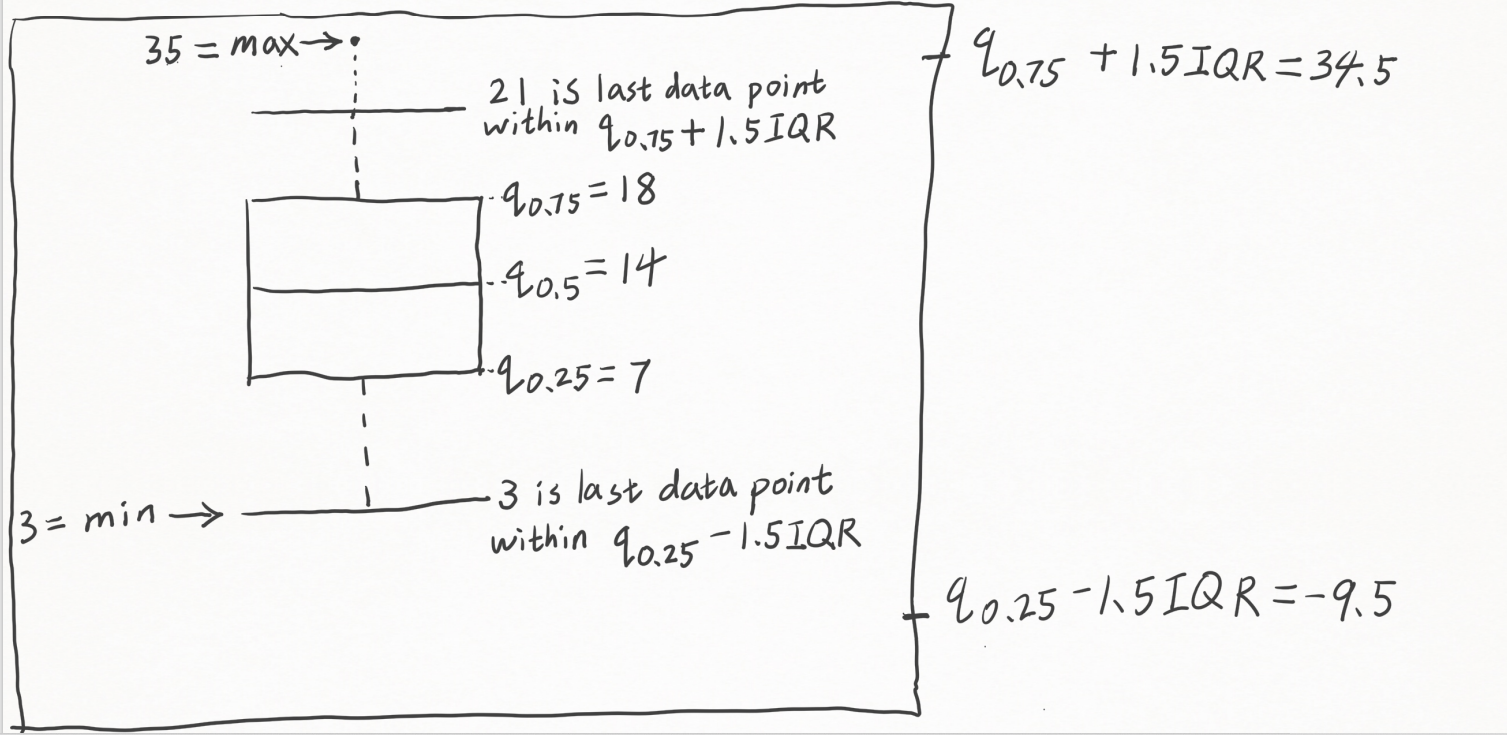
\includegraphics[width=1.3\textwidth, height=0.8\textwidth]{1} %img size
\end{figure}
\newpage
\noindent
Problem 2\\
1.\\
$T_1$ is unbiased, so $E[T_1] = \theta\\
E[W] = 0\\
T_2 = T_1 + W\\
E[T_2] = E[T_1 + W] = E[T_1] + E[W] = \theta + 0 = \theta\\$
$E[T_2] = \theta$, so $T_2$ is an unbiased estimator for $\theta$\\
\\
\\
\\
2.\\
\begin{align*}
E[T_2] &= E\left[\frac{T_1 - b}{a}\right]\\
&= \frac{1}{a}E[T_1 - b]\\
&= \frac{1}{a}(E[T_1] - E[b])\\ 
&= \frac{1}{a}(E[T_1] - b)\quad\text{/* since $b$ is a constant */}\\
&= \frac{1}{a}(a\theta + b - b)\\
&= \frac{1}{a}(a\theta)\\
&= \theta
\end{align*}
$E[T_2] = \theta$, so $T_2$ is an unbiased estimator for $\theta$\\
\newpage
\noindent
Problem 3\\
uniform distribution probability density function $f$ is\\
{\large
$f(x) = 
\begin{cases}
0 & \text{if } x \not \in [a, b]\\
\frac{1}{b - a} & \text{if } x \in [a, b]\\
\end{cases}\\
\\
f_X(x) = 
\begin{cases}
0 & \text{if } x \not \in [0, \theta]\\
1 / \theta & \text{if } x \in [0, \theta]\\
\end{cases}\\
\text{if } x \in [0, \theta], \; F_X(x) = \int_0^x f_X(x) dx = \int_0^x \frac{1}{\theta} dx = \frac{1}{\theta}\int_0^x dx = \frac{x}{\theta}\\
F_X(x) = 
\begin{cases}
0 & \text{if } x \not \in [0, \theta]\\
x / \theta & \text{if } x \in [0, \theta]\\
\end{cases}\\$}
\begin{align*}
F_T(t) = P(T \leq t) &= P(X_1 \leq t, X_2 \leq t, ..., X_n \leq t)\\
&= \prod_{i = 1}^n P(X_i \leq t)\\
&= \prod_{i = 1}^n F_{X_i}(t)\\
&= \prod_{i = 1}^n \left(\frac{t}{\theta}\right)\\
&= \left(\frac{t}{\theta}\right)^n\\
\end{align*}
\begin{align*}
f_T(t) &= \frac{d}{dt}(F_T(t))\\ 
&= \frac{d}{dt}\left(\left(\frac{t}{\theta}\right)^n\right)\\
&= n \left(\frac{t}{\theta}\right)^{n - 1}\left(\frac{1}{\theta}\right)\\
\end{align*}
\begin{center}
{\large
$f_T(t) = 
\begin{cases}
0 & \text{if } t \not\in [0, \theta]\\
n \left(\frac{t}{\theta}\right)^{n - 1}\left(\frac{1}{\theta}\right) & \text{if } t \in [0, \theta]\\
\end{cases}$}
\end{center}
\begin{align*}
E[T] &= \int_0^\theta t f_T(t) dt\\
&= \int_0^\theta t \left(n\left(\frac{t}{\theta}\right)^{n - 1}\left(\frac{1}{\theta}\right)\right) dt\\
&= \frac{n}{\theta^n} \int_0^\theta t^n dt\\ 
&= \frac{n}{\theta^n} \left[\frac{t^{n + 1}}{n + 1}\right]_0^\theta\\
&= \frac{n}{\theta^n} \frac{\theta^{n + 1}}{n + 1}\\
&= \frac{n}{n + 1}\theta\\
\end{align*}
\begin{align*}
B(T) &= E[T] - \theta\\
&= \frac{n}{n + 1}\theta - \theta\\
&= \frac{n\theta - (n + 1)\theta}{n + 1}\\
&= \frac{n\theta - n\theta - \theta}{n + 1}\\
&= \boxed{-\frac{\theta}{n + 1}}\\
\end{align*}
\newpage
\noindent
Problem 4\\
1.\\
probability to respond yes = probability of responding yes without lying + probability of responding yes with lying = $\frac{1}{6}\mu + \frac{5}{6}(1 - \mu) = \frac{5}{6} - \frac{4}{6}\mu$\\
probability to respond no = probability of responding no without lying + probability of responding no with lying = $\frac{1}{6}(1 - \mu) + \frac{5}{6}\mu = \frac{1}{6} + \frac{4}{6}\mu$\\
{\large
$X_i = \begin{cases}
1 & \text{if the response is yes}\\
0 & \text{if the response is no}\\
\end{cases}\\
\boxed{
P(X_i = x) = \begin{cases}
\frac{5}{6} - \frac{4}{6}\mu & \text{if } x = 1\\
\frac{1}{6} + \frac{4}{6}\mu & \text{if } x = 0\\
\end{cases}}\\
\\
P(X_i = x) = \begin{cases}
p & \text{if } x = 1\\
1 - p & \text{if } x = 0\\
\end{cases}\\
E[X_i] = 1 \cdot p + 0 \cdot (1 - p) = p = \frac{5}{6} - \frac{4}{6}\mu$}
\newpage
\noindent
2.\\
\begin{align*}
E[T_n] &= E\left[\frac{5}{4} - \frac{3}{2}\overline{X_n}\right]\\
&= \frac{5}{4} - \frac{3}{2}E[\overline{X_n}]\\
&= \frac{5}{4} - \frac{3}{2}E\left[\frac{\sum_{i = 1}^n X_i}{n}\right]\\
&= \frac{5}{4} - \frac{3}{2}\frac{1}{n}\sum_{i = 1}^n E\left[X_i\right]\\
&= \frac{5}{4} - \frac{3}{2}\frac{n}{n} E[X_i]\\
&= \frac{5}{4} - \frac{3}{2} E[X_i]\\
&= \frac{5}{4} - \frac{3}{2} p\\
&= \frac{5}{4} - \frac{3}{2} \left(\frac{5}{6} - \frac{4}{6}\mu\right)\\
&= \frac{5}{4} - \frac{5}{4} + \mu\\
&= \mu\\
\end{align*}
$E[T_n] = \mu$, so $T_n$ is an unbiased estimator for $\mu$\\
\newpage
\noindent
3. 
\begin{align*}
Var(T_n) &= Var\left[\frac{5}{4} - \frac{3}{2}\overline{X_n}\right]\\
&= Var\left[-\frac{3}{2}\overline{X_n}\right]\\
&= \left(-\frac{3}{2}\right)^2 Var(\overline{X_n})\\
&= \frac{9}{4}Var(\overline{X_n})\\
&= \frac{9}{4}Var\left(\frac{\sum_{i = 1}^n X_i}{n}\right)\\
&= \frac{9}{4n^2}Var(\sum_{i = 1}^n X_i)\\
&= \frac{9}{4n^2}\sum_{i = 1}^n Var(X_i)\\
&= \frac{9n}{4n^2} Var(X_i)\\
&= \frac{9}{4n} Var(X_i)\\
&= \frac{9}{4n} p(1 - p)\\
&= \frac{9}{4n} (\frac{5}{6} - \frac{4}{6}\mu)(1 - (\frac{5}{6} - \frac{4}{6}\mu))\\
&= \frac{9}{4n} (\frac{5}{6} - \frac{4}{6}\mu)(\frac{1}{6} + \frac{4}{6}\mu)\\
&= \frac{9}{4n} (\frac{5}{36} + \frac{20}{36}\mu - \frac{4}{36}\mu - \frac{16}{36}\mu^2)\\
&= \frac{9}{4n} (\frac{5}{36} + \frac{16}{36}\mu - \frac{16}{36}\mu^2)\\
&= \frac{9}{144n} (5 + 16\mu - 16\mu^2)\\
&= \boxed{\frac{45}{144n} + \frac{\mu}{n} - \frac{\mu^2}{n}}\\
\end{align*}
\newpage
\noindent
Problem 5\\
1.\\
likelihood function $L(\theta)$ is
\begin{align*}
L(\theta) &= f_{\theta, X_1, X_2, ..., X_n} (a_1, a_2, ..., a_n)\\
&= \prod_{i = 1}^n f_\theta (a_i)\\
&= \prod_{i = 1}^n \frac{2}{\sqrt{\pi}\theta^{3 / 2}} a_i^2 e^{-a_i^2 / \theta}\\
&= \left(\frac{2}{\sqrt{\pi}\theta^{3 / 2}}\right)^n \left(\prod_{i = 1}^n a_i^2 \right) e^{-\sum_{i = 1}^n a_i^2 / \theta}\\
\end{align*}
loglikelihood function $l(\theta)$ is
\begin{align*}
l(\theta) &= \ln(L(\theta))\\
&= \ln\left(\left(\frac{2}{\sqrt{\pi}\theta^{3 / 2}}\right)^n \left(\prod_{i = 1}^n a_i^2 \right) e^{-\sum_{i = 1}^n a_i^2 / \theta}\right)\\
&= \ln\left(\left(\frac{2}{\sqrt{\pi}\theta^{3 / 2}}\right)^n\right) + \ln\left(\prod_{i = 1}^n a_i^2 \right) + \ln\left(e^{-\sum_{i = 1}^n a_i^2 / \theta}\right)\\
&= n\ln\left(\frac{2}{\sqrt{\pi}\theta^{3 / 2}}\right) + \left(\sum_{i = 1}^n\ln(a_i^2)\right) -\sum_{i = 1}^n a_i^2 / \theta\\
\end{align*}
\begin{align*}
\frac{dl}{d\theta} &= (-3 / 2)\frac{2}{\sqrt{\pi}}\theta^{-5 / 2} n \frac{1}{2 / (\sqrt{\pi}\theta^{3 / 2})} + \sum_{i = 1}^n a_i^2 / \theta^2\\
&= \frac{-3}{\sqrt{\pi}}\theta^{-5 / 2} n \frac{\sqrt{\pi}\theta^{3 / 2}}{2} + \sum_{i = 1}^n a_i^2 / \theta^2\\
&= \frac{-3n}{2\theta} + \sum_{i = 1}^n a_i^2 / \theta^2\\
\end{align*}\\
\begin{align*}
\frac{dl}{d\theta} &= 0\\
\frac{-3n}{2\theta} + \sum_{i = 1}^n a_i^2 / \theta^2 &= 0\\
\frac{-3n}{2\theta} + \frac{1}{\theta^2}\sum_{i = 1}^n a_i^2 &= 0\\
\frac{1}{\theta^2}\sum_{i = 1}^n a_i^2 &= \frac{3n}{2\theta}\\
\frac{1}{\theta}\sum_{i = 1}^n a_i^2 &= \frac{3n}{2}\\
\frac{1}{\theta} &= \frac{3n}{2\sum_{i = 1}^n a_i^2}\\
\theta &= \frac{2\sum_{i = 1}^n a_i^2}{3n}\\
\end{align*}
so the maximum likelihood estimate of $\theta$ is
\[\theta_m = \frac{2\sum_{i = 1}^n a_i^2}{3n}\]
\newpage
\noindent
2.\\
\begin{align*}
bias(\hat{\theta}) &= E[\hat{\theta}] - \theta
\end{align*}
\begin{align*}
E[\hat{\theta}] &= E\left[\frac{2\sum_{i = 1}^n x_i^2}{3n}\right]\\
&= \frac{2}{3n}E[\sum_{i = 1}^n x_i^2]\\
&= \frac{2}{3n}\sum_{i = 1}^n E[x_i^2]\\
\end{align*}
\begin{align*}
E[x^2] &= \int_{-\infty}^{\infty} x^2 f_\theta(x) dx\\
&= \int_{-\infty}^{\infty} x^2 \left(\frac{2}{\sqrt{\pi}\theta^{3 / 2}} x^2 e^{-x^2 / \theta}\right) dx\\
&= \frac{2}{\sqrt{\pi}\theta^{3 / 2}} \int_{-\infty}^{\infty} x^4 e^{-x^2 / \theta} dx\\
\end{align*}
to calculate $\int_{-\infty}^{\infty} x^4 e^{-x^2 / \theta} dx$:\\ 
a continuous random variable has a normal distribution with parameters $\mu$ and $\sigma^2 > 0$ if its probability density function is given by
{\large
\begin{align*}
f(x) &= \frac{1}{\sqrt{2\pi\sigma^2}} e^{-\frac{1}{2}\left(\frac{x - \mu}{\sigma}\right)^2}\\
\end{align*}}
\begin{align*}
\int_{-\infty}^{\infty} f(x) dx &= \int_{-\infty}^{\infty} \frac{1}{\sqrt{2\pi\sigma^2}} e^{-\frac{1}{2}\left(\frac{x - \mu}{\sigma}\right)^2} dx\\
&= \frac{1}{\sqrt{2\pi\sigma^2}} \int_{-\infty}^{\infty} e^{-\frac{1}{2}\left(\frac{x - \mu}{\sigma}\right)^2} dx\\
\text{/* set } \mu = 0; \qquad K &= \frac{1}{2\sigma^2}; \qquad \sigma = \frac{1}{\sqrt{2K}} \text{*/}\\
&= \frac{1}{\sqrt{2\pi(1/\sqrt{2K})^2}} \int_{-\infty}^{\infty} e^{-\frac{1}{2}\left(\frac{x - 0}{1/(\sqrt{2K})}\right)^2} dx\\
&= \frac{1}{\sqrt{2\pi}(1/\sqrt{2K})} \int_{-\infty}^{\infty} e^{-\frac{1}{2}\left(\sqrt{2K}x\right)^2} dx\\
&= \frac{\sqrt{2K}}{\sqrt{2\pi}} \int_{-\infty}^{\infty} e^{-\frac{1}{2}\left(2Kx^2\right)} dx\\
&= \sqrt{\frac{K}{\pi}} \int_{-\infty}^{\infty} e^{-Kx^2} dx = 1\\
\text{/* since } \int_{-\infty}^{\infty} f(x)dx  = 1 &\text{ for a $f$ that is the probability density}\\
&\text{function of a continuous random variable $X$}\text{ */}\\
\int_{-\infty}^{\infty} e^{-Kx^2} dx &= \sqrt{\frac{\pi}{K}}\\
\end{align*}
\begin{align*}
I(K) := \int_{-\infty}^{\infty} e^{-Kx^2} dx &= \sqrt{\frac{\pi}{K}} = \sqrt{\pi}K^{-1 / 2}\\
\frac{\partial I}{\partial K} = \int_{-\infty}^{\infty} (-x^2)e^{-Kx^2} dx &= -\frac{\sqrt{\pi}}{2}K^{-3 / 2}\\
\frac{\partial^2 I}{\partial K^2} = \int_{-\infty}^{\infty} x^4 e^{-Kx^2} dx &= \frac{3\sqrt{\pi}}{4}K^{-5 / 2}\\
\text{/* set } K = \frac{1}{\theta} \text{ */}\\
\int_{-\infty}^{\infty} x^4 e^{-x^2 / \theta} dx &= \frac{3\sqrt{\pi}}{4}\left(\frac{1}{\theta}\right)^{-5 / 2}
= \frac{3\sqrt{\pi}}{4}\theta^{5 / 2}\\
\end{align*}
return to calculate $E[x^2]$
\begin{align*}
E[x^2] &= \frac{2}{\sqrt{\pi}\theta^{3 / 2}} \int_{-\infty}^{\infty} x^4 e^{-x^2 / \theta} dx\\
&= \frac{2}{\sqrt{\pi}\theta^{3 / 2}} \left(\frac{3\sqrt{\pi}}{4}\theta^{5 / 2}\right)\\
&= \frac{3}{2}\theta\\
\end{align*}
return to calculate $bias(\hat{\theta})$
\begin{align*}
bias(\hat{\theta}) &= E[\hat{\theta}] - \theta\\
&= \frac{2}{3n}\left(\sum_{i = 1}^n E[x_i^2]\right) - \theta\\
&= \frac{2}{3n}\left(\sum_{i = 1}^n \frac{3}{2}\theta\right) - \theta\\
&= \frac{1}{n}(n\theta) - \theta\\
&= \theta - \theta\\
&= \boxed{0}\\
\end{align*}
\newpage
\noindent
3.
\begin{align*}
Var(\hat{\theta}) &= Var\left(\frac{2\sum_{i = 1}^n x_i^2}{3n}\right)\\
&= \frac{4}{9n^2}Var(\sum_{i = 1}^n x_i^2)\\
&= \frac{4}{9n^2}\sum_{i = 1}^n Var(x_i^2)\\
&= \frac{4}{9n^2}\sum_{i = 1}^n \left(E[(x_i^2)^2] - E[x_i^2]^2\right)\\
&= \frac{4}{9n^2}\sum_{i = 1}^n \left(E[x_i^4] - E[x_i^2]^2\right)\\
\end{align*}
\begin{align*}
E[x^4] &= \int_{-\infty}^{\infty} x^4 f_\theta(x) dx\\
&= \int_{-\infty}^{\infty} x^4 \left(\frac{2}{\sqrt{\pi}\theta^{3 / 2}} x^2 e^{-x^2 / \theta}\right) dx\\
&= \frac{2}{\sqrt{\pi}\theta^{3 / 2}} \int_{-\infty}^{\infty} x^6 e^{-x^2 / \theta} dx\\
\end{align*}
to calculate $\int_{-\infty}^{\infty} x^6 e^{-x^2 / \theta} dx$:\\
from Problem 5. 2 it is shown that 
\begin{align*}
\frac{\partial^2 I}{\partial K^2} = \int_{-\infty}^{\infty} x^4 e^{-Kx^2} dx &= \frac{3\sqrt{\pi}}{4}K^{-5 / 2}\\
\frac{\partial^3 I}{\partial K^3} = \int_{-\infty}^{\infty} -x^6 e^{-Kx^2} dx &= -\frac{15\sqrt{\pi}}{8}K^{-7 / 2}\\
\end{align*}
\begin{align*}
\int_{-\infty}^{\infty} x^6 e^{-Kx^2} dx &= \frac{15\sqrt{\pi}}{8}K^{-7 / 2}\\
\text{/* set } K &= \frac{1}{\theta} \text{ */}\\
\int_{-\infty}^{\infty} x^6 e^{-x^2 / \theta} dx &= \frac{15\sqrt{\pi}}{8}\left(\frac{1}{\theta}\right)^{-7 / 2}\\
&= \frac{15\sqrt{\pi}}{8}\theta^{7 / 2}\\
\end{align*}
return to calculate $E[x^4]$
\begin{align*}
E[x^4] &= \frac{2}{\sqrt{\pi}\theta^{3 / 2}} \int_{-\infty}^{\infty} x^6 e^{-x^2 / \theta} dx\\
&= \frac{2}{\sqrt{\pi}\theta^{3 / 2}} \left(\frac{15\sqrt{\pi}}{8}\theta^{7 / 2}\right)\\
&= \frac{15}{4}\theta^2\\
\end{align*}
return to calculate $Var(\hat{\theta})$
\begin{align*}
Var(\hat{\theta}) &= \frac{4}{9n^2}\sum_{i = 1}^n \left(E[x_i^4] - E[x_i^2]^2\right)\\
&= \frac{4}{9n^2}\sum_{i = 1}^n \left(\frac{15}{4}\theta^2 - \left(\frac{3}{2}\theta\right)^2\right)\\
&= \frac{4}{9n^2}\sum_{i = 1}^n \left(\frac{15}{4}\theta^2 - \frac{9}{4}\theta^2\right)\\
&= \frac{4}{9n^2}\sum_{i = 1}^n \left(\frac{6}{4}\theta^2\right)\\
&= \frac{2}{3n^2}\sum_{i = 1}^n \theta^2\\
&= \frac{2n}{3n^2}\theta^2\\
&= \frac{2}{3n}\theta^2\\
\end{align*}
as one increases the number $n$ of independent observations, $Var(\hat{\theta})$ decreases since there is a $n$ in the denominator\\
\end{document}